% to do:

\documentclass[mathserif]{beamer}
\usetheme{Boadilla}
\usepackage{lmodern}
%\input{style.tex}
%gets rid of bottom navigation bars
\setbeamertemplate{footline}{}
%gets rid of navigation symbols
\setbeamertemplate{navigation symbols}{}

\usepackage{xcolor}
\usepackage{array}
\usepackage{setspace}
\usepackage{animate}
\usepackage{verbatim}
\usepackage{svg}
\usepackage{amsmath}
\usepackage{bm}
\usepackage{algorithm, algorithmic}

\definecolor{dkred}{rgb}{0.8,0,0}
\definecolor{dkgreen}{rgb}{0,0.6,0}


\linespread{1}
\setbeamerfont{frametitle}{size=\normalsize}
\setbeamercolor{alerted text}{fg=blue,bg=white}

%\setbeamersize{text margin left=5pt,text margin right=5pt}

\DeclareMathOperator{\y}{y}

\DeclareMathOperator{\td}{\mathrm{d}}
\def\E{{\mathbb E}}
\def\R{{\mathbb R}}

\DeclareMathOperator{\xvec}{\mathbf{x}}
\DeclareMathOperator{\yvec}{\mathbf{y}}
\DeclareMathOperator{\fvec}{\mathbf{f}}
\DeclareMathOperator{\uvec}{\mathbf{u}}
\DeclareMathOperator{\Bcal}{\mathcal{B}}
\DeclareMathOperator{\Norm}{\mathcal{N}}
\DeclareMathOperator{\muvec}{\boldsymbol{\mu}}
\DeclareMathOperator{\Sigvec}{\boldsymbol{\Sigma}}
\DeclareMathOperator{\Kvec}{\mathbf{K}}

\DeclareMathOperator{\by}{\bm{\mathrm{y}}}


\newcommand{\appropto}{\mathrel{\vcenter{
  \offinterlineskip\halign{\hfil$##$\cr
    \propto\cr\noalign{\kern2pt}\sim\cr\noalign{\kern-2pt}}}}}
\newcommand*{\bigCI}{%
  \mathrel{\text{%
    {\rotatebox[origin=c]{90}{\resizebox{2.25ex}{1.65ex}{$\vDash$}}}%
  }}%
}

\newcommand{\argmax}[1]{\underset{#1}{\operatorname{arg}\,\operatorname{max}}\;}
\newcommand{\argmin}[1]{\underset{#1}{\operatorname{arg}\,\operatorname{min}}\;}

\setbeamertemplate{itemize items}[default]
\setbeamertemplate{enumerate items}[default]


%\usepackage[style=authoryear,maxcitenames=2,uniquelist=false,doi=false,isbn=false,url=false]{biblatex}
%\renewcommand*{\bibfont}{\footnotesize}
%\usepackage[style=numeric-comp,sorting=none,uniquelist=false,doi=false,isbn=false,url=false]{biblatex}
%\addbibresource{ref.bib}

\title[Stochastic Expectation Propagation]{Stochastic Expectation Propagation}
\subtitle{}
\author{Yingzhen Li and Rich Turner }
\renewcommand{\author}[1]{}
%\institute{CBL, Cambridge}
%\date{Oct 6th, 2014}

\begin{document}
\maketitle
%

%%%%%%%%%%%%%%%%%%%%%%%%%%%%%%%%%%%%%%%%%%%%%%%%%%%%%%%%%%

\begin{frame}{Introducing Expectation Propagation (EP)}

 Approximate Bayesian parameter learning
\begin{equation}
{\color{dkred}p(\bm{\theta} | \mathcal{D})} \propto {\color{dkred}p_0(\bm{\theta}) \prod_{n=1}^{N} p(\bm{x}_n | \bm{\theta})} \uncover<2->{\approx {\color{dkgreen} q(\bm{\theta})} \propto {\color{dkgreen}p_0(\bm{\theta}) \prod_{n=1}^{N} f_n(\bm{\theta})}\nonumber}
\end{equation}

\uncover<2->{ \textbf{Goal:} ${\color{dkgreen}f_n(\bm{\theta})} \approx$ effect likelihood term ${\color{dkred}p(\bm{x}_n | \bm{\theta}) }$ has on posterior}\\
\vspace{3mm}
\uncover<3->{ \textbf{Idea 1:}  $\argmin{\color{dkgreen}f_n(\theta)} \mathrm{KL}[{\color{dkred}p(\bm{\theta}|\mathcal{D})} || {\color{dkred}p(\bm{\theta}|\mathcal{D})} {\color{dkgreen} f_n(\bm{\theta})}/ {\color{dkred}p(\bm{x}_n | \bm{\theta})}]$}
\vspace{3mm}

\uncover<4->{ \textbf{Idea 2:}  bootstrap: replace leave-one-out posterior on both sides by approximate leave-one-out posterior}
%
\uncover<4->{ \begin{equation}
\mathrm{KL}[ {\color{dkred}p_{-n}(\bm{\theta}) p(\bm{x}_n| \bm{\theta})} ||  {\color{dkred} p_{-n}(\bm{\theta})} {\color{dkgreen} f_n(\bm{\theta})}] \uncover<6->{\approx \mathrm{KL}[ {\color{dkgreen} q_{-n}(\bm{\theta})} {\color{dkred} p(\bm{x}_n | \bm{\theta})} ||  {\color{dkgreen} q_{-n}(\bm{\theta}) f_n(\bm{\theta})}]} \nonumber
\end{equation}}
%
\vspace{-4mm}
%
\uncover<4->{
\begin{equation}
{\color{dkred} p_{-n}(\bm{\theta})} \propto {\color{dkred} p(\bm{\theta}|\mathcal{D})} / {\color{dkred}p(\bm{x}_n | \bm{\theta})} \uncover<5->{ \approx {\color{dkgreen} q_{-n}(\bm{\theta})} \propto {\color{dkgreen}q(\bm{\theta})}/{\color{dkgreen}f_n(\bm{\theta})}}\nonumber
\end{equation}}


\uncover<7->{  updates now coupled $\implies$ iterate until convergence }
\end{frame}

%%%%%%%%%%%%%%%%%%%%%%%%%%%%%%%%%%%%%%%%%%%%%%%%%%%%%%%%%%%%%%%%%%%%%%%%%%%%

\begin{frame}{EP algorithm}

\begin{figure}[!t]
% UGLY USE OF \vspace & \hspace follows
\begin{minipage}[t]{0.45\linewidth}
\centering
\begin{algorithm}[H] 
\renewcommand{\thealgorithm}{}
\caption{EP} 
\label{alg:ep} 
\begin{algorithmic}[1] 
	\STATE  choose factor $f_n$ to refine:
	\STATE compute cavity distribution \\$q_{-n}(\bm{\theta}) \propto q(\bm{\theta}) / f_n(\bm{\theta})$ 
	\STATE compute tilted distribution \\$\tilde{p}_n(\bm{\theta}) \propto p(\bm{x}_n|\bm{\theta}) q_{-n}(\bm{\theta})$
	\STATE moment matching: \\ \hspace{-1mm}$f_n(\bm{\theta}) \leftarrow \mathtt{proj}[\tilde{p}_n(\bm{\theta})] / q_{-n}(\bm{\theta}) $
	\STATE inclusion:\\ $q(\bm{\theta}) \leftarrow q_{-n}(\bm{\theta}) f_n(\bm{\theta})$\\\hspace{1mm}\\ \vspace{1.5mm} \hspace{1mm}\\
\end{algorithmic}
\end{algorithm}
\end{minipage}
%
\uncover<2->{\begin{minipage}[t]{0.45\linewidth}
\centering
\begin{itemize}
\item[]
\item[]
\item[+] {\color{dkgreen} reduces to classical algorithms in special cases (loopy BP, Kalman filter, ...)}
\item[-] {\color{dkred}few theoretical guarantees (convergence, evidence bounds, ...)}
\item[+] {\color{dkgreen} computation local to each factor}
\item[-] {\uncover<3->{\textbf{}\color{dkred}number of approximating factors $\propto N$} \uncover<3->{}}
\end{itemize}
\end{minipage}}

%
%\caption{Comparing the Expectation Propagation (EP), Assumed Density Filtering (ADF), and Stochastic Expectation Propagation (SEP) update steps. Typically, the algorithms will be initialised using $q(\bm{\theta}) = p_0(\bm{\theta})$ and, where appropriate, $f_n(\bm{\theta})=1$ or $f(\bm{\theta})=1$.}
\end{figure}
\end{frame}

%%%%%%%%%%%%%%%%%%%%%%%%%%%%%%%%%%%%%%%%%%%%%%%%%%%%%%%%%%%%%%%%%%%%%%%%%%%%

\begin{frame}{EP and ADF}

\begin{figure}[!t]
% UGLY USE OF \vspace & \hspace follows
\begin{minipage}[t]{0.45\linewidth}
\centering
\begin{algorithm}[H] 
\renewcommand{\thealgorithm}{}
\caption{EP} \small
\label{alg:ep} 
\begin{algorithmic}[1] 
	\STATE \small choose factor $f_n$ to refine:
	\STATE compute cavity distribution \\${\color{dkgreen}q_{-n}(\bm{\theta}) \propto q(\bm{\theta}) / f_n(\bm{\theta})}$ 
	\STATE compute tilted distribution \\$\tilde{p}_n(\bm{\theta}) \propto p(\bm{x}_n|\bm{\theta}) q_{-n}(\bm{\theta})$
	\STATE moment matching: \\ \hspace{-1mm}$f_n(\bm{\theta}) \leftarrow \mathtt{proj}[\tilde{p}_n(\bm{\theta})] / q_{-n}(\bm{\theta}) $
	\STATE inclusion:\\ $q(\bm{\theta}) \leftarrow q_{-n}(\bm{\theta}) f_n(\bm{\theta})$\\\hspace{1mm}\\ \vspace{1.5mm} \hspace{1mm}\\
\end{algorithmic}
\end{algorithm}
\end{minipage}
%
\begin{minipage}[t]{0.45\linewidth}
\centering
\begin{algorithm}[H] 
\renewcommand{\thealgorithm}{}
\caption{ADF} \small
\label{alg:adf} 
\begin{algorithmic}[1] 
	\STATE \small choose a datapoint $\bm{x}_n\sim \mathcal{D}$:
	\STATE compute cavity distribution \\${\color{red}q_{-n}(\bm{\theta}) = q(\bm{\theta})}$
	\STATE compute tilted distribution \\$\tilde{p}_n(\bm{\theta}) \propto p(\bm{x}_n|\bm{\theta}) q_{-n}(\bm{\theta})$
	\STATE moment matching: \\ \hspace{-1mm}$f_n(\bm{\theta}) \leftarrow \mathtt{proj}[\tilde{p}_n(\bm{\theta})] / q_{-n}(\bm{\theta}) $
	\STATE inclusion:\\ $q(\bm{\theta}) \leftarrow q_{-n}(\bm{\theta}) f_n(\bm{\theta})$\\\hspace{1mm}\\ \vspace{1.5mm} \hspace{1mm}\\
\end{algorithmic}
\end{algorithm}
\end{minipage}
%
%\caption{Comparing the Expectation Propagation (EP), Assumed Density Filtering (ADF), and Stochastic Expectation Propagation (SEP) update steps. Typically, the algorithms will be initialised using $q(\bm{\theta}) = p_0(\bm{\theta})$ and, where appropriate, $f_n(\bm{\theta})=1$ or $f(\bm{\theta})=1$.}
\end{figure}

\uncover<2->{
\begin{itemize}
\item[+] {\color{dkgreen} only maintain global approximation (retain local computation)}
\item[-] {\color{dkred} posterior variance shrinks to zero (overfits, not Bayesian)}
\end{itemize}}

\end{frame}
%%%%%%%%%%%%%%%%%%%%%%%%%%%%%%%%%%%%%%%%%%%%%%%%%%%%%%%%%%%%%%%%%%%%%%%%%%%%


\begin{frame}{SEP idea}

Approximate Bayesian parameter learning

\begin{equation}
{\color{dkred}p(\bm{\theta} | \mathcal{D})} \propto {\color{dkred}p_0(\bm{\theta}) \prod_{n=1}^{N} p(\bm{x}_n | \bm{\theta})} \approx {\color{dkgreen} q(\bm{\theta})} \propto {\color{dkgreen}p_0(\bm{\theta}) \prod_{n=1}^{N} f_n(\bm{\theta})}\nonumber
\end{equation}

At convergence EP factors parameterise a global approximation that represents the average effect of a likelihood term on the posterior

\begin{equation}
 {\color{dkgreen}p_0(\bm{\theta}) \prod_{n=1}^{N} f_n(\bm{\theta})} = {\color{dkgreen}p_0(\bm{\theta})  f(\bm{\theta})^{N}}\nonumber
\end{equation}

\uncover<2->{\textbf{Idea:} work with ${\color{dkgreen}f(\bm{\theta})}$  directly}
\end{frame}


%\begin{frame}{SEP}
%
%
%\begin{equation}
%{\color{dkred}p(\bm{\theta} | \mathcal{D})} \propto {\color{dkred}p_0(\bm{\theta}) \prod_{n=1}^{N} p(\bm{x}_n | \bm{\theta})} \uncover<2->{\approx {\color{dkgreen} q(\bm{\theta})} \propto {\color{dkgreen}p_0(\bm{\theta})  f(\bm{\theta})^{N}}\nonumber}
%\end{equation}
%
%\uncover<2->{ \textbf{Goal:} ${\color{dkgreen}f(\bm{\theta})} \approx$ average effect one likelihood term $\{ {\color{dkred}p(\bm{x}_n | \bm{\theta}) } \}_{n=1}^N$ has on posterior}\\
%\vspace{3mm}
%\uncover<4->{ \textbf{Idea:} treat $f(\bm{\theta})$}
%%
%\uncover<4->{ \begin{equation}
%\mathrm{KL}[ {\color{dkred}p_{-n}(\bm{\theta}) p(\bm{x}_n| \bm{\theta})} ||  {\color{dkred} p_{-n}(\bm{\theta})} {\color{dkgreen} f_n(\bm{\theta})}] \uncover<6->{\approx \mathrm{KL}[ {\color{dkgreen} q_{-n}(\bm{\theta})} {\color{dkred} p(\bm{x}_n | \bm{\theta})} ||  {\color{dkgreen} q_{-n}(\bm{\theta}) f_n(\bm{\theta})}]} \nonumber
%\end{equation}}
%%
%\vspace{-4mm}
%%
%\uncover<4->{
%\begin{equation}
%{\color{dkred} p_{-n}(\bm{\theta})} \propto {\color{dkred} p(\bm{\theta}|\mathcal{D})} / {\color{dkred}p(\bm{x}_n | \bm{\theta})} \uncover<5->{ \approx {\color{dkgreen} q_{-n}(\bm{\theta})} \propto {\color{dkgreen}q(\bm{\theta})}/{\color{dkgreen}f_n(\bm{\theta})}}\nonumber
%\end{equation}}
%
%
%\uncover<7->{  updates now coupled $\implies$ iterate until convergence }
%\end{frame}
%

%%%%%%%%%%%%%%%%%%%%%%%%%%%%%%%%%%%%%%%%%%%%%%%%%%%%%%%%%%%%%%%%%%%%%%%%%%%%

\begin{frame}{EP vs SEP}

\begin{figure}[!t]
% UGLY USE OF \vspace & \hspace follows
\begin{minipage}[t]{0.45\linewidth}
\centering
\begin{algorithm}[H]
\renewcommand{\thealgorithm}{} 
\caption{EP} \small
\label{alg:ep} 
\begin{algorithmic}[1] 
	\STATE \small choose factor $f_n$ to refine:
	\STATE compute cavity distribution \\ $\color{dkgreen}q_{-n}(\bm{\theta}) \propto q(\bm{\theta}) / f_n(\bm{\theta})$ 
	\STATE compute tilted distribution \\$\tilde{p}_n(\bm{\theta}) \propto p(\bm{x}_n|\bm{\theta}) q_{-n}(\bm{\theta})$
	\STATE moment matching: \\ \hspace{-1mm}$f_n(\bm{\theta}) \leftarrow \mathtt{proj}[\tilde{p}_n(\bm{\theta})] / q_{-n}(\bm{\theta}) $
	\STATE inclusion:\\ $q(\bm{\theta}) \leftarrow q_{-n}(\bm{\theta}) f_n(\bm{\theta})$\\\hspace{1mm}\\ \vspace{1.5mm} \hspace{1mm}\\
\end{algorithmic}
\end{algorithm}
\end{minipage}
%\quad
\begin{minipage}[t]{0.45\linewidth}
\centering
\begin{algorithm}[H]
\renewcommand{\thealgorithm}{}
\caption{SEP} \small
\label{alg:sep} 
\begin{algorithmic}[1] 
%\STATE initialize $\{\tilde{f}_a\}$
	\STATE \small choose a datapoint $\bm{x}_n\sim \mathcal{D}$:
	\STATE compute cavity distribution \\ $\color{dkgreen}q_{-1}(\bm{\theta}) \propto q(\bm{\theta}) / f(\bm{\theta})$
	\STATE compute tilted distribution \\$\tilde{p}_n(\bm{\theta}) \propto p(\bm{x}_n|\bm{\theta}) q_{-1}(\bm{\theta})$
	\STATE moment matching: \\\hspace{-1mm}$f_n(\bm{\theta}) \leftarrow \mathtt{proj}[\tilde{p}_n(\bm{\theta})] / q_{-1}(\bm{\theta}) $
	\STATE inclusion:\\ $q(\bm{\theta}) \leftarrow q_{-1}(\bm{\theta}) f_n(\bm{\theta})$
	\STATE {\color{blue}\textit{implicit update}:\\ $f(\bm{\theta}) \leftarrow f(\bm{\theta})^{1 - \frac{1}{N}} f_n(\bm{\theta})^{\frac{1}{N}}$}
\end{algorithmic}
\end{algorithm}
\end{minipage} 
\end{figure}
\end{frame}
%%%%%%%%%%%%%%%%%%%%%%%%%%%%%%%%%%%%%%%%%%%%%%%%%%%%%%%%%%%%%%%%%%%%%%%%%%%%


\begin{frame}{EP vs ADF}

\begin{figure}[!t]
% UGLY USE OF \vspace & \hspace follows
\begin{minipage}[t]{0.45\linewidth}
\centering
\begin{algorithm}[H] 
\renewcommand{\thealgorithm}{}
\caption{ADF} \small
\label{alg:adf} 
\begin{algorithmic}[1] 
	\STATE \small choose a datapoint $\bm{x}_n\sim \mathcal{D}$:
	\STATE compute cavity distribution \\$\color{dkred}q_{-n}(\bm{\theta}) = q(\bm{\theta})$
	\STATE compute tilted distribution \\$\tilde{p}_n(\bm{\theta}) \propto p(\bm{x}_n|\bm{\theta}) q_{-n}(\bm{\theta})$
	\STATE moment matching: \\ \hspace{-1mm}$f_n(\bm{\theta}) \leftarrow \mathtt{proj}[\tilde{p}_n(\bm{\theta})] / q_{-n}(\bm{\theta}) $
	\STATE inclusion:\\ $q(\bm{\theta}) \leftarrow q_{-n}(\bm{\theta}) f_n(\bm{\theta})$\\\hspace{1mm}\\ \vspace{1.5mm} \hspace{1mm}\\
\end{algorithmic}
\end{algorithm}
\end{minipage}
%\quad
\begin{minipage}[t]{0.45\linewidth}
\centering
\begin{algorithm}[H]
\renewcommand{\thealgorithm}{}
\caption{SEP} \small
\label{alg:sep} 
\begin{algorithmic}[1] 
%\STATE initialize $\{\tilde{f}_a\}$
	\STATE \small choose a datapoint $\bm{x}_n\sim \mathcal{D}$:
	\STATE compute cavity distribution \\ $\color{dkgreen}q_{-1}(\bm{\theta}) \propto q(\bm{\theta}) / f(\bm{\theta})$
	\STATE compute tilted distribution \\$\tilde{p}_n(\bm{\theta}) \propto p(\bm{x}_n|\bm{\theta}) q_{-1}(\bm{\theta})$
	\STATE moment matching: \\\hspace{-1mm}$f_n(\bm{\theta}) \leftarrow \mathtt{proj}[\tilde{p}_n(\bm{\theta})] / q_{-1}(\bm{\theta}) $
	\STATE inclusion:\\ $q(\bm{\theta}) \leftarrow q_{-1}(\bm{\theta}) f_n(\bm{\theta})$
	\STATE {\color{blue} \textit{implicit update}:\\ $f(\bm{\theta}) \leftarrow f(\bm{\theta})^{1 - \frac{1}{N}} f_n(\bm{\theta})^{\frac{1}{N}}$}
\end{algorithmic}
\end{algorithm}
\end{minipage} 
\end{figure}
\end{frame}
%%%%%%%%%%%%%%%%%%%%%%%%%%%%%%%%%%%%%%%%%%%%%%%%%%%%%%%%%%%%%%%%%%%%%%%%%%%%




\begin{frame}{Classification (Probit): synthetic data }
  \begin{overprint}
   \onslide<1>\centerline{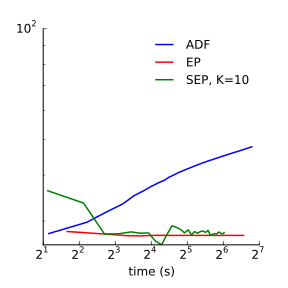
\includegraphics[width=7cm]{figs/sep_probit}}
 \end{overprint}
\end{frame}
%%%%%%%%%%%%%%%%%%%%%%%%%%%%%%%%%%%%%%%%%%%%%%%%%%%%%%%%%%%%%%%%%%%%%%%%%%%%


\begin{frame}{Classification (Probit): real data }
  \begin{overprint}
   \onslide<1>\centerline{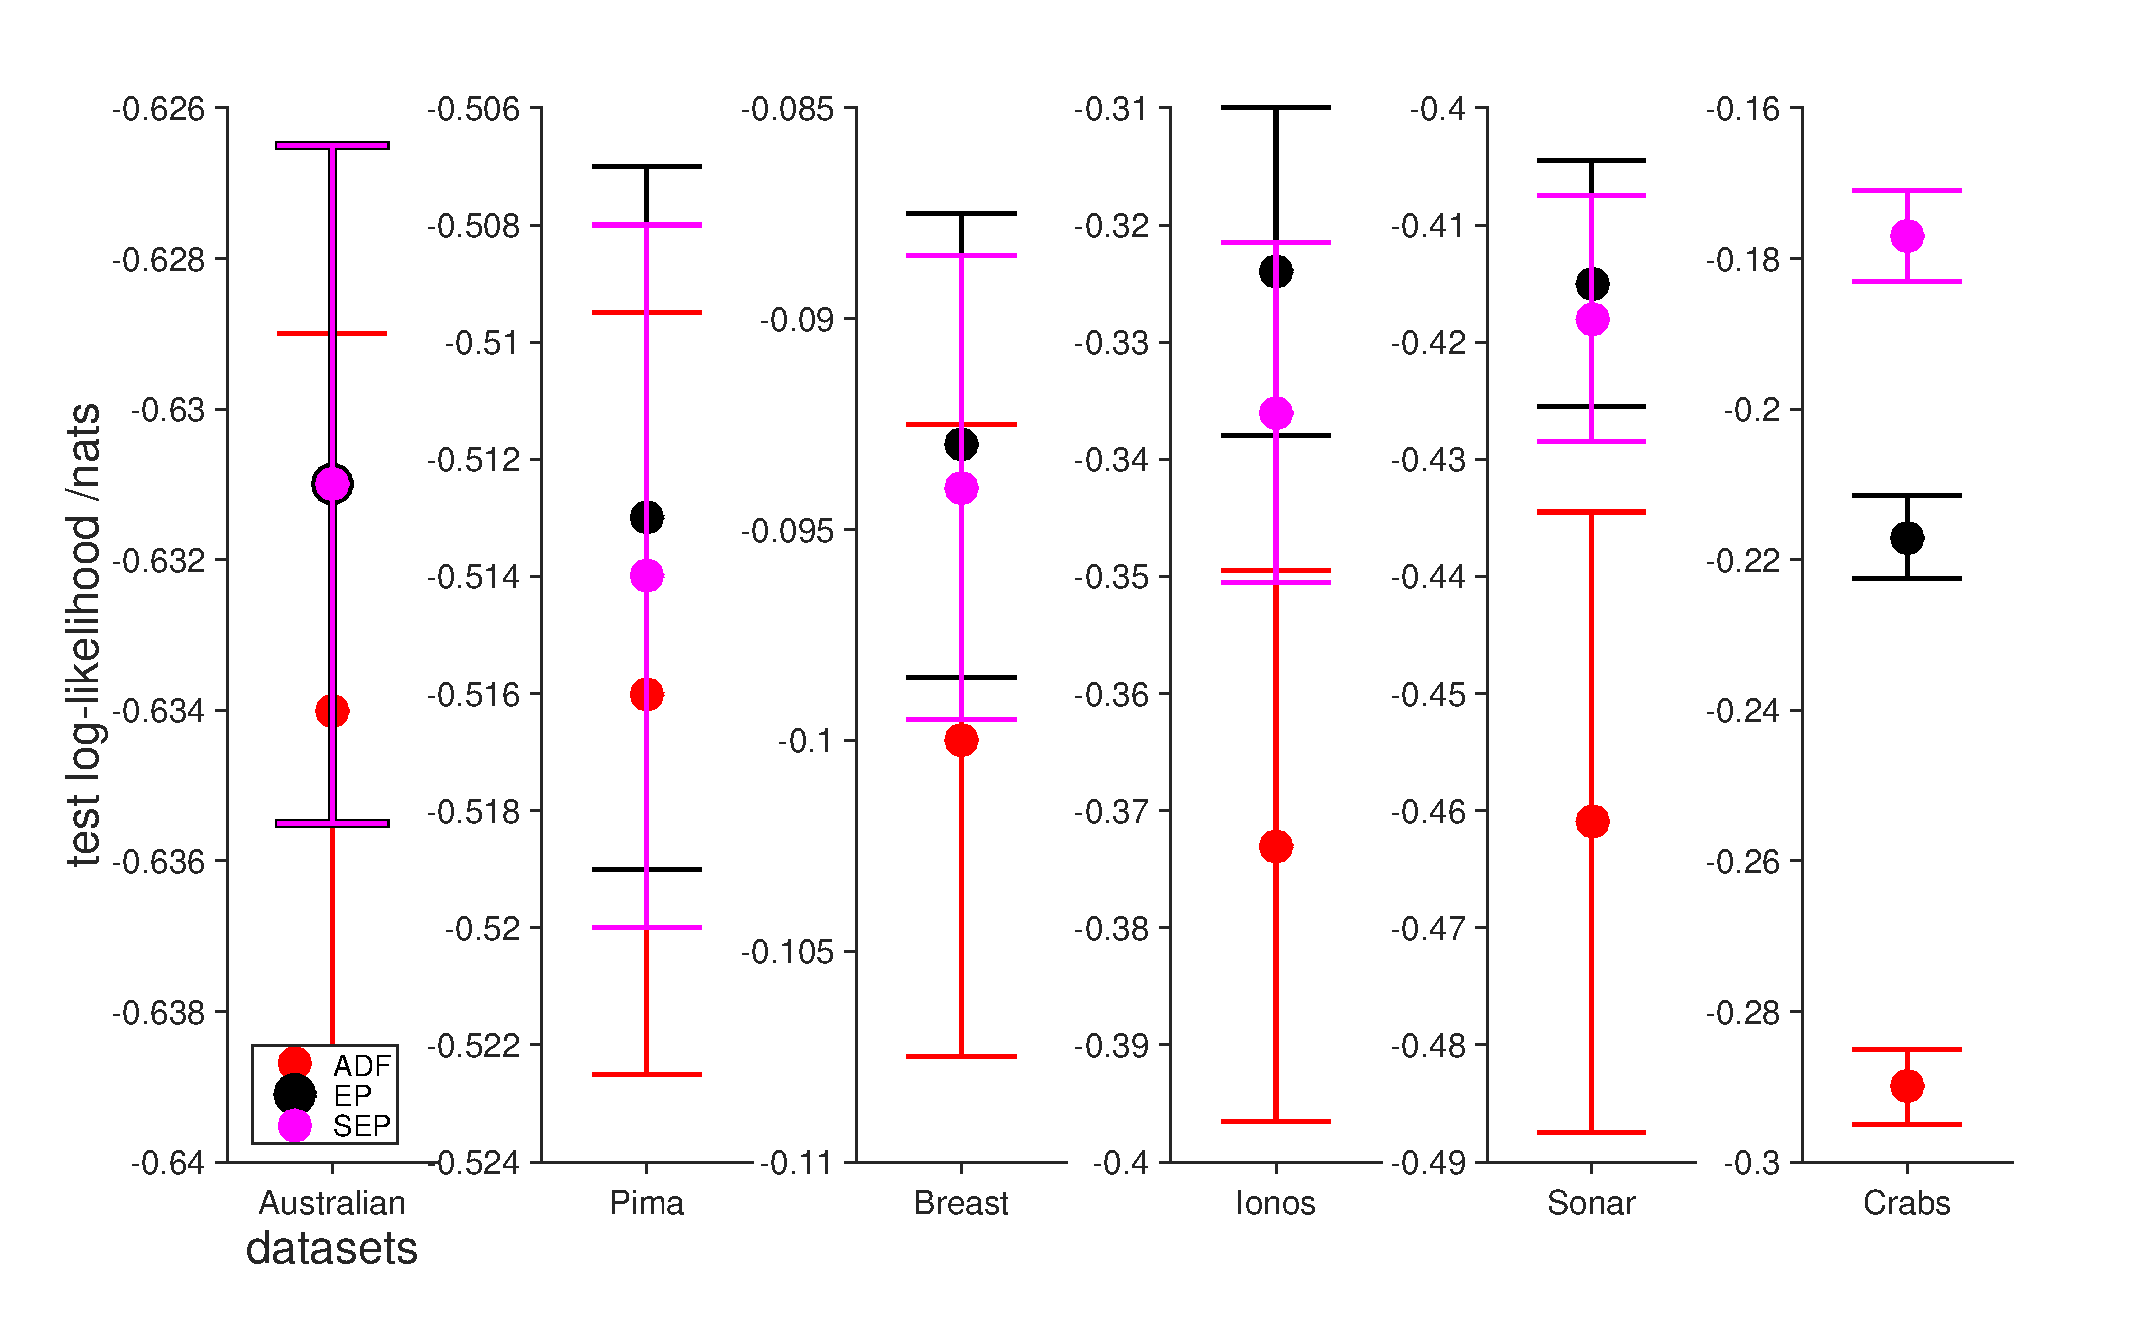
\includegraphics[width=10cm]{figs/sep_probit_real_data}}
  \end{overprint}
\end{frame}

%%%%%%%%%%%%%%%%%%%%%%%%%%%%%%%%%%%%%%%%%%%%%%%%%%%%%%%%%%%%%%%%%%%%%%%%%%%%

\begin{frame}{Gaussian Mixture Model: synthetic data }
  \begin{overprint}
   \onslide<1>\centerline{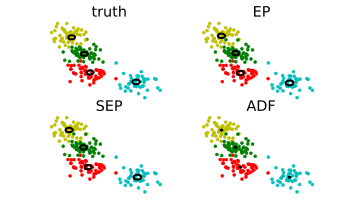
\includegraphics[width=9cm]{figs/gmm1}}
  \end{overprint}
  
\end{frame}
\begin{frame}{Gaussian Mixture Model: synthetic data }
  \begin{overprint}
   \onslide<1>\centerline{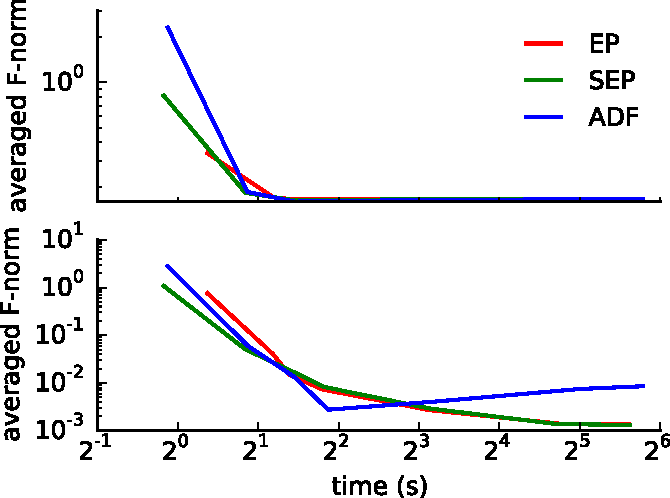
\includegraphics[width=9cm]{figs/gmm_error}}
  \end{overprint}
\end{frame}
%%%%%%%%%%%%%%%%%%%%%%%%%%%%%%%%%%%%%%%%%%%%%%%%%%%%%%%%%%%%%%%%%%%%%%%%%%%%


\begin{frame}{Classification (Probit): real data }
  \begin{overprint}
   \onslide<1>\centerline{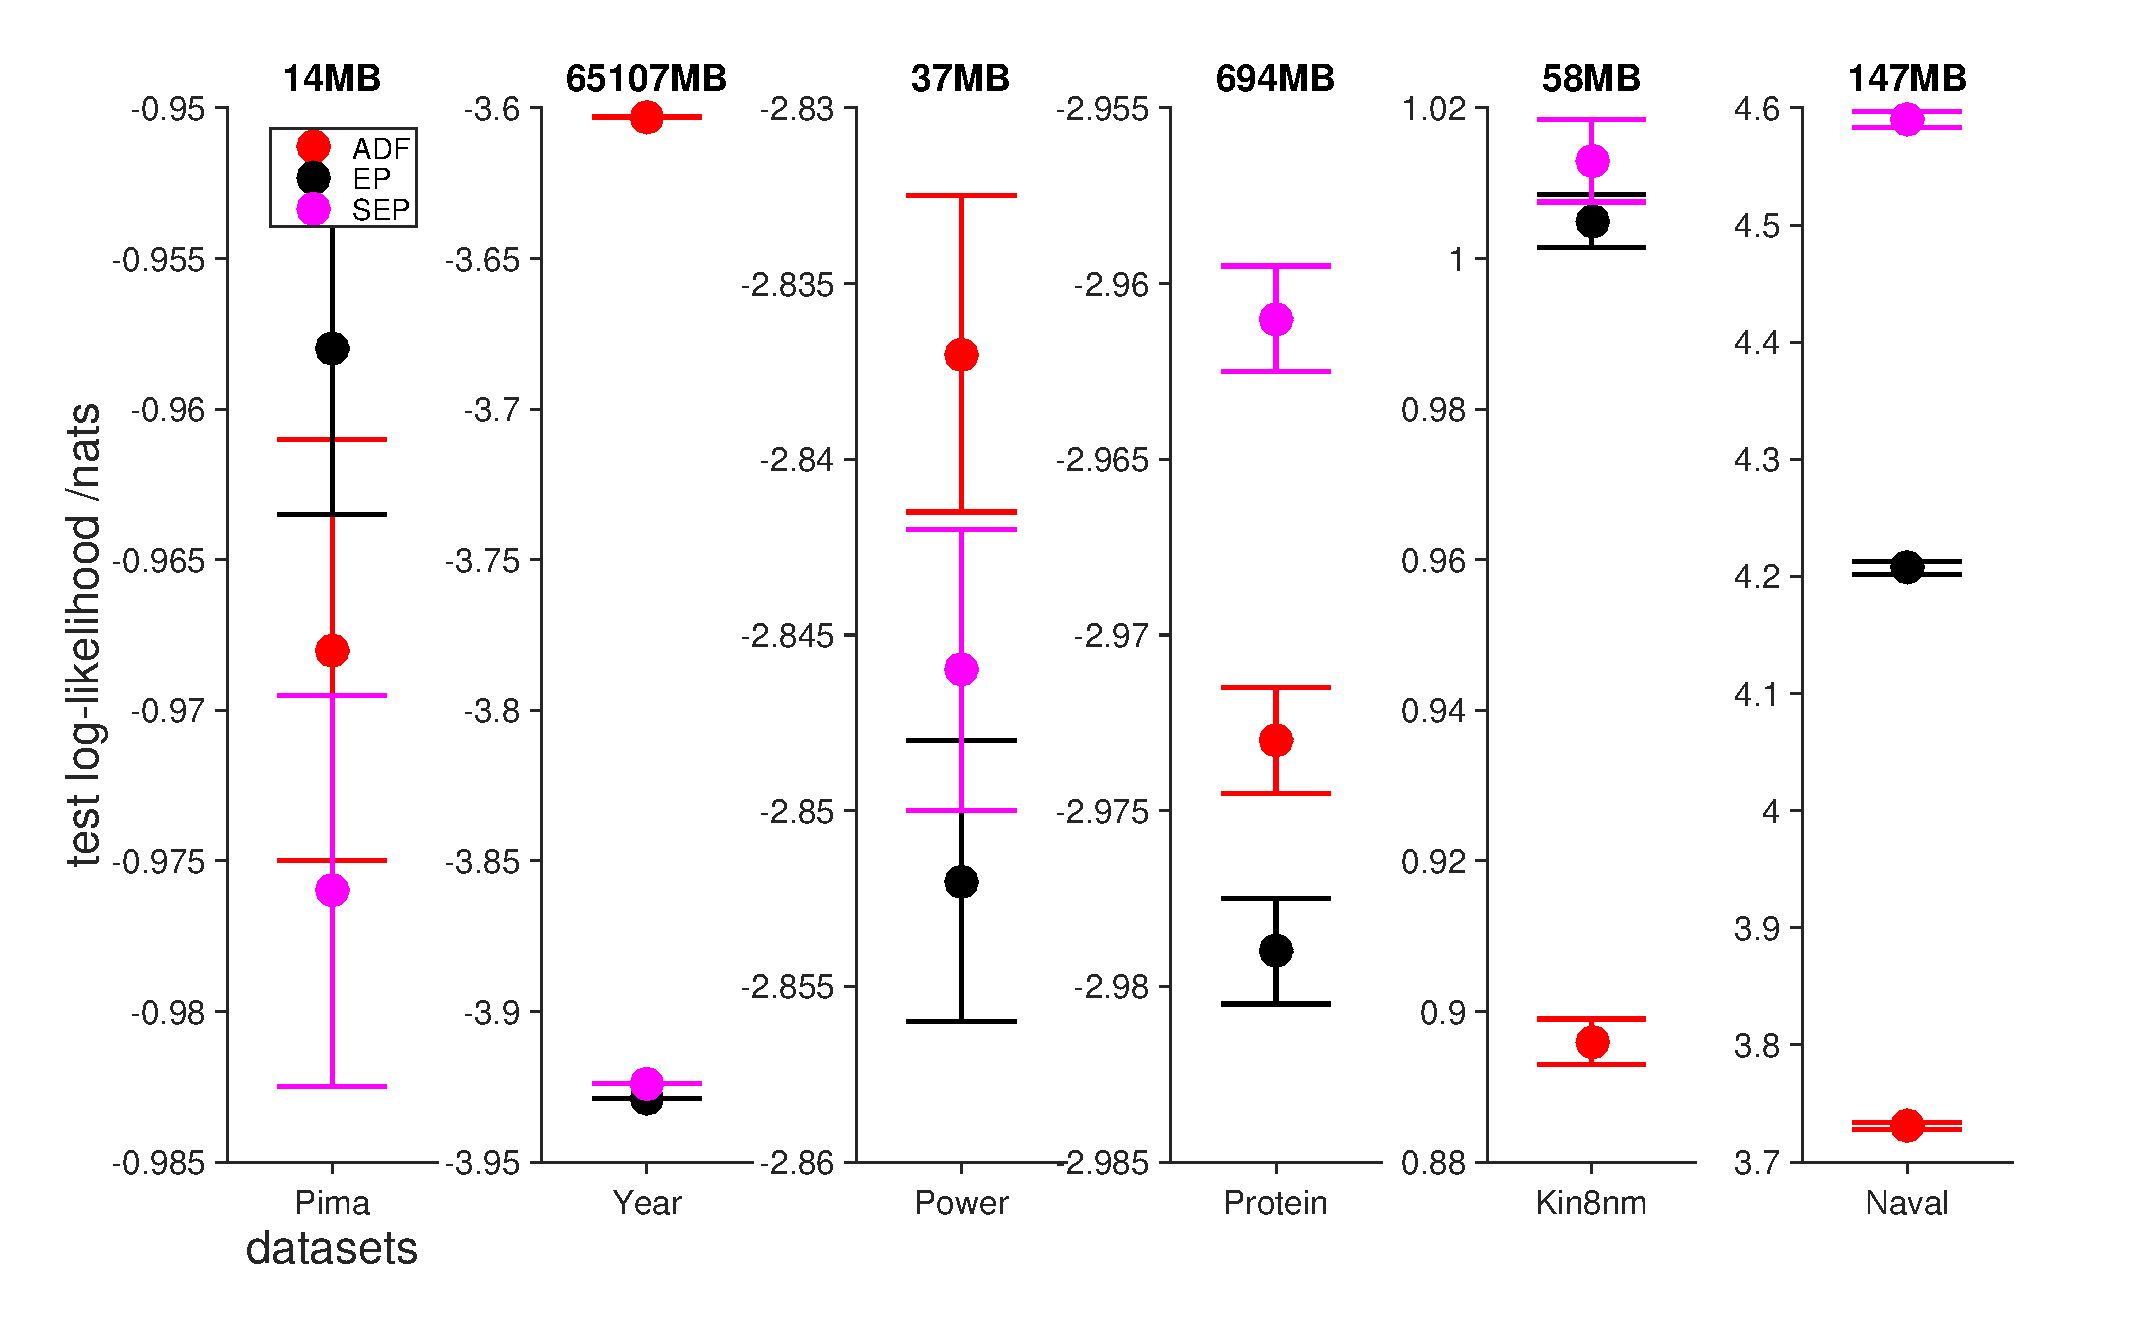
\includegraphics[width=10cm]{figs/sep_dnn_real_data}}
  \end{overprint}
\end{frame}
%%%%%%%%%%%%%%%%%%%%%%%%%%%%%%%%%%%%%%%%%%%%%%%%%%%%%%%%%%%%%%%%%%%%%%%%%%%%

\begin{frame}{Conclusions, extensions, open questions}
\begin{itemize}
\item \textbf{typically}:\\ {\color{blue}\textbf{SEP performs almost as well as EP w/ N-fold memory reduction  }}
\item \textbf{theory}: same fixed points as EP (in expectation) under certain conditions, same fixed points (in expectation) as variational methods if $\text{KL}(q||p)$ used
\item \textbf{generalisations}: can use less coarse approximation ($M$ approximating factors, SEP uses $M=1$, EP uses $M=N$)
\item \uncover<2->{\color{dkred}\textbf{Critical open question for EP enterprise:} Is EP \textbf{ever} better than variational methods? }
\end{itemize}
\end{frame}

%%%%%%%%%%%%%%%%%%%%%%%%%%%%%%%%%%%%%%%%%%%%%%%%%%%%%%%%%%%%%%%%%%%%%%%%%%%%


\begin{frame}{Relationship with other algorithms}
  \begin{overprint}
   \onslide<1>\centerline{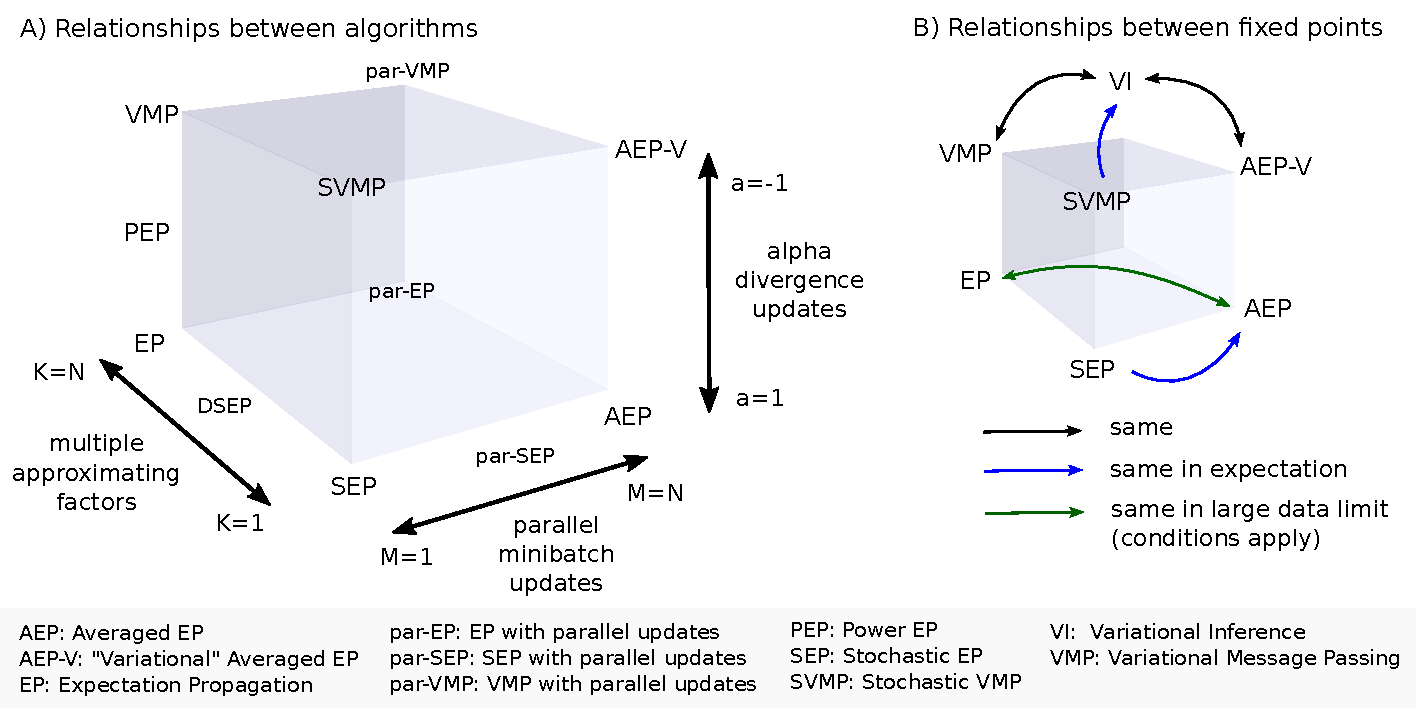
\includegraphics[width=12cm]{figs/relationship-algorithms}}
  \end{overprint}
\end{frame}


\end{document}
